% enable opacity in l3opacity
\DocumentMetadata{}
\documentclass{article}
\usepackage[margin=3.5cm]{geometry}
\usepackage[T1]{fontenc}
\usepackage{xcolor}
\usepackage{amsmath}
\usepackage{graphicx}
\usepackage{l3draw}
\usepackage{l3opacity}
\usepackage{framed}


\newcommand{\next}{\vspace*{4em}\par}

\title{l3draw Learn}
\author{Eureka}
\date{\today}
\begin{document}
\maketitle
\tableofcontents
\section{Basic}
\subsection{unit}
Default unit of l3draw is \textbf{pt}.


\subsection{How to displace in Doc}
Except for function \verb|\draw_path_use_clear:n {}|, all the other functions don't display 
anything on screen.


\subsection{polar point}
\begin{align}
  (\rho, \theta) & \leftrightarrow (\rho\cos\theta, \rho\sin\theta) \\
  (\rho_1, \rho_2, \theta)& \leftrightarrow (\rho_1\cos\theta, \rho_2\sin\theta)
\end{align}


\subsection{base vectors}
The \verb|\draw_x(y)vec:n| defines 2 base vectors that can be used in command \verb|\draw_point_vec:nn|.
So the \verb|\draw_xvec:n| returns nothing, but the \verb|\draw_point_vec:nn| returns a coodinate. The standard
base is \textbf{1cm} in $x(y)$ direction.

All \textbf{vec}-based command is \textbf{relative} to the above defined $x(y)-$vectors. That's 
if you changed the base, the norm of \verb|\draw_point_vec_polar:nn {1}{0}|= $\|e_x\|$, while that 
of \verb|\draw_point_polar:nn {1}{0}| $\equiv$ 1pt. 

\subsection{root}
The \verb|{root}| in commands related to intersection is a \textbf{integer}, reprensent the index of the intersection(s).

\subsection{interpolation}
Return a point the \verb|<part>|-way of the line between the two points \verb|<point1>| and \verb|<point2>|.
Then \verb|<part>| would be a float value.

Or you can use distance instead of portion. The distance is the \textbf{absolutely} value of the distance
to the \textbf{first} point(point-1). see below figure \ref{fig:distance}:
\begin{figure}[!htb]
    \centering
    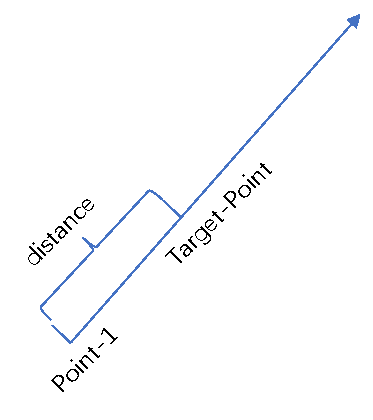
\includegraphics[width=.4\linewidth]{./distance.pdf}
    \caption{distance}
    \label{fig:distance}
\end{figure}

% \ExplSyntaxOn
% \draw_begin:
%   \moveto:n {0, 0}
%   % how to draw a brace in l3draw ?
% \draw_end:
% \ExplSyntaxOff



\section{Path}
arc length = (corner) to (the point curve start). \textbf{leading in}:from the previous path operation.
so does the \textbf{leading out}.

Make a path close, use command \verb|\draw_path_close:|, contrast to \verb|--cycle| in tikz.

\subsection{show path}
To show a path you can use command \verb|\draw_path_use:n|, using the following action:
\begin{itemize}
  \item stroke(draw)
  \item fill 
  \item clip
\end{itemize}

You can also clear the path after show it, using command \verb|\draw_path_use_clear:n| instead.

\subsection{replace bounding box}
Replaces the current bounding box of the drawing with one specified by the current path, which means 
this bb \textbf{won't update in the future}. For that ``All functions automatically update the bounding 
box of the image'', unless specified \verb|\l_draw_bb_update_bool=false|.

\subsection{canva}
canvas-related functions ignore the transformation matrix.

\subsection{Phase in Path pattern}
What is the ``phase'' in \verb|\draw_dash_pattern:nn |? Remeber that \textbf{left:+, right:-}.

\vspace*{2em}
\noindent\textcolor{red}{The ⟨phase⟩} \textcolor{blue}{specifies} (that) 
the pattern should start \textcolor{orange}{where} \textcolor{gray}{during the first 'on' line}

\noindent The ⟨phase⟩ specifies where (during the first “on” line) the pattern should start.

\subsection{fill rule}
there are 2 rules to check whether a region is ``internal'' of a path:
\begin{itemize}
  \item \textbf{Non-zero winding number rule}
  \item \textbf{Even-odd rule}
\end{itemize}

\section{box in drawing}
box in l3draw, like `node' in tikz.It takes account of the current transformation matrix
and shift. But you can use `xcoffins' to re-set it to the original box.


\section{transform matrix}
\verb|\draw_transform_matrix:nnnn {a}{b}{c}{d}| corresponding to a matrix(denoted by $T$) below:
\begin{align}
  T = 
  \begin{bmatrix}
    a & c \\
    b & d
  \end{bmatrix}
\end{align}

that's ``arranged column by column''. You can \textbf{shift, scale, rotate, slant} the drawing using pre-defined 
functions. But all the functions are juse special cases to the previous transformation matrix.

\subsection{invert and reset}
\textbf{invert} applys the inverse of current transforming matrix to the drawing, that is applying the 
following matrix:
% inverse matrix of 
\begin{align}
  T = \frac{1}{ad-bc}
  \begin{bmatrix}
    d & -c \\
    -b & a
  \end{bmatrix}
\end{align}

Whilst, \textbf{reset} means: reset the current transforming matrix to the identity matrix, that is 
\begin{align}
  T = 
  \begin{bmatrix}
    1 & 0 \\
    0 & 1
  \end{bmatrix}
\end{align}


\section{scope and layers}
layers is important in drawing. Default layer is \verb|main|. Create a new layer using \verb|\draw_layer_new:n {newlayer}|,
then use it in scope \verb|\draw_layer_begin:n {newlayer} <draw code>\draw_layer_end:|.

Note that each scope or layer loacl environment should have a \verb|\draw_path_use:n {}| function to show the scope 
drawing material.

\section{Draw style}
\subsection{draw path action}
you can \textbf{draw(stroke), fill, clip} a path, thus you can specify the color of the path using
\verb|\color_fill:n| or \verb|\color_stroke:n|. The stroke color will apply to both \textbf{path} and 
\textbf{text} in the drawing.

\subsection{opacity}
To support ``opacity'' in l3draw, add \verb|\DocumentMetadata{}| before \verb|\documentclass{}|


\section{Implement}
\subsection{function plot}
{
\scriptsize
\begin{framed}
\begin{verbatim}
% ===> function plot and shade command
% \function_plot:nnn {<function>}{<domain>}{<style>}
% functin = {<function>}
% domain = {<x-start>, <x-step>, <x-end>, <y-min>, <y-max>}
% style = {<unit>, <action>, <color-1>, <color-2>, <gradient-axis>}
\cs_generate_variant:Nn \fp_step_inline:nnnn {eeen}
\cs_set:Npn \function_plot:nnn #1#2#3 {
  % => split arg
  \args_split_cs:nn {#2}{domain}
  \args_split_cs:nn {#3}{style}
  % => draw function 
  \draw_begin:
    % normal part
    \str_case:VnT \l__arg_style_ii {
      {stroke}{\exp_args:Nx \color_stroke:n {\tl_use:N \l__arg_style_iii}}
      {draw}{\exp_args:Nx \color_stroke:n {\tl_use:N \l__arg_style_iii}}
      {fill}{\exp_args:Nx \color_fill:n {\tl_use:N \l__arg_style_iii}}
      {clip}{\relax}
    }{
      % => start point
      \tl_set:Nn \l_tmpa_tl {#1}
      \tl_replace_all:Nne \l_tmpa_tl {x}{(\tl_use:N \l__arg_domain_i)}
      \draw_path_moveto:n {\l__arg_domain_i\l__arg_style_i, \l_tmpa_tl\l__arg_style_i}
      % loop to draw path
      \fp_step_inline:eeen {\l__arg_domain_i}{\l__arg_domain_ii}{\l__arg_domain_iii}{
          \tl_set:Nn \l_tmpa_tl {#1}
          \tl_replace_all:Nnn \l_tmpa_tl {x}{(##1)}
          \draw_path_lineto:n {##1 \l__arg_style_i, \l_tmpa_tl \l__arg_style_i}
      }
      \draw_path_use_clear:n {\l__arg_style_ii}
    }
    % shade plot part
    \str_if_eq:VnT \l__arg_style_ii {shade}{
      % start and end point for 'y-axis gradient'
      \tl_if_eq:VnT \l__arg_style_v {y}{
        \tl_if_exist:cF {l__start_tl}{
          \tl_new:N \l__start_tl
          \tl_new:N \l__end_tl
        } 
        \tl_set:Nx \l__start_tl {\l__arg_domain_iv}
        \tl_set:Nx \l__end_tl {\l__arg_domain_v}
      }
      % loop to plot segements
      \fp_step_inline:eeen {\l__arg_domain_i}{\l__arg_domain_ii}{\fp_eval:n {\l__arg_domain_iii-\l__arg_domain_ii}}{
          \tl_set:Nn \l_tmpa_tl {#1}
          \tl_set:Nn \l_tmpb_tl {#1}
          \tl_replace_all:Nnn \l_tmpa_tl {x}{(##1)}
          \tl_replace_all:Nnn \l_tmpb_tl {x}{(##1+\l__arg_domain_ii)}
          \str_case:VnF \l__arg_style_v {
            {x}{\color_gradient:xxx {
                \fp_eval:n {(##1-\l__arg_domain_i)*(100/(\l__arg_domain_iii-\l__arg_domain_i))}
              }{\l__arg_style_iii}{\l__arg_style_iv}}
            {y}{\color_gradient:xxx {
                \fp_eval:n {(\l_tmpa_tl-\l__start_tl)*(100/(\l__end_tl-\l__start_tl))}
              }{\l__arg_style_iii}{\l__arg_style_iv}}
          }{\relax}
          \draw_path_moveto:n {##1 \l__arg_style_i, \l_tmpa_tl \l__arg_style_i}
          \draw_path_lineto:n {(##1+\l__arg_domain_ii) \l__arg_style_i, \l_tmpb_tl \l__arg_style_i}
          % \draw_cap_rectangle:
          \draw_cap_round:
          \draw_path_use_clear:n {draw}
      }
    }
  \draw_end:
}

% args split 
\cs_generate_variant:Nn \int_step_inline:nnn {nen}
\cs_generate_variant:Nn \seq_set_split:Nnn {cnn}
\cs_set:Npn \args_split_cs:nn #1#2 {
  \seq_if_exist:cF {l_#2_seq}{
    \seq_new:c {l_#2_seq}
  }
  \seq_set_split:cnn {l_#2_seq}{,}{#1}
  \int_step_inline:nen {1}{\seq_count:c {l_#2_seq}}{
    \tl_set:Nn \l_tmpa_tl {l__arg_#2_\int_to_roman:n{##1}}
    \exp_args:Nfo \tl_if_exist:cF {\tl_use:N \l_tmpa_tl}{
      \tl_new:c {\tl_use:N \l_tmpa_tl}
    }
    \tl_set:ce {\tl_use:N \l_tmpa_tl}{\seq_item:cn {l_#2_seq}{##1}}
  }
}

% color gradient
\cs_set:Npn \color_gradient:nnn #1#2#3 {
  \fp_compare:nNnTF {#1}>{100}{
    \exp_args:Nx \color_select:n {#2!\fp_eval:n{abs(#1)/(\l__arg_domain_v-\l__arg_domain_iv)}!#3} 
  }{
    \fp_compare:nNnTF {#1}<{0}{
      \exp_args:Nx \color_select:n {#2!\fp_eval:n{abs(#1)/(\l__arg_domain_v-\l__arg_domain_iv)}!#3} 
    }{\color_select:n {#2!#1!#3}}
  }
}
\cs_generate_variant:Nn \color_gradient:nnn {xxx}

\function_plot:nnn {x^3-2*x}{-5, 0.25, 5, -1, 1}{em, shade, blue, green, x}
% \function_plot:nnn {x^3-2*x}{-3, 1, 3, -1, 1}{em, draw, blue, green, x}
% \function_plot:nnn {sin(x)}{0, 0.02*\c_pi_fp, 2*\c_pi_fp, -1, 1}{em, shade, blue, green, y}
\end{verbatim}
\end{framed}
}


\subsection{Shade plot}


\section{l3 Draw Example}
\centering
\ExplSyntaxOn
% ===> function plot and shade command
% \function_plot:nnn {<function>}{<domain>}{<style>}
% functin = {<function>}
% domain = {<x-start>, <x-step>, <x-end>, <y-min>, <y-max>}
% style = {<unit>, <action>, <color-1>, <color-2>, <gradient-axis>}
\cs_generate_variant:Nn \fp_step_inline:nnnn {eeen}
\cs_set:Npn \function_plot:nnn #1#2#3 {
  % => split arg
  \args_split_cs:nn {#2}{domain}
  \args_split_cs:nn {#3}{style}
  % => draw function 
  \draw_begin:
    % normal part
    \str_case:VnT \l__arg_style_ii {
      {stroke}{\exp_args:Nx \color_stroke:n {\tl_use:N \l__arg_style_iii}}
      {draw}{\exp_args:Nx \color_stroke:n {\tl_use:N \l__arg_style_iii}}
      {fill}{\exp_args:Nx \color_fill:n {\tl_use:N \l__arg_style_iii}}
      {clip}{\relax}
    }{
      % => start point
      \tl_set:Nn \l_tmpa_tl {#1}
      \tl_replace_all:Nne \l_tmpa_tl {x}{(\tl_use:N \l__arg_domain_i)}
      \draw_path_moveto:n {\l__arg_domain_i\l__arg_style_i, \l_tmpa_tl\l__arg_style_i}
      % loop to draw path
      \fp_step_inline:eeen {\l__arg_domain_i}{\l__arg_domain_ii}{\l__arg_domain_iii}{
          \tl_set:Nn \l_tmpa_tl {#1}
          \tl_replace_all:Nnn \l_tmpa_tl {x}{(##1)}
          \draw_path_lineto:n {##1 \l__arg_style_i, \l_tmpa_tl \l__arg_style_i}
      }
      \draw_path_use_clear:n {\l__arg_style_ii}
    }
    % shade plot part
    \str_if_eq:VnT \l__arg_style_ii {shade}{
      % start and end point for 'y-axis gradient'
      \tl_if_eq:VnT \l__arg_style_v {y}{
        \tl_if_exist:cF {l__start_tl}{
          \tl_new:N \l__start_tl
          \tl_new:N \l__end_tl
        } 
        \tl_set:Nx \l__start_tl {\l__arg_domain_iv}
        \tl_set:Nx \l__end_tl {\l__arg_domain_v}
      }
      % loop to plot segements
      \fp_step_inline:eeen {\l__arg_domain_i}{\l__arg_domain_ii}{\fp_eval:n {\l__arg_domain_iii-\l__arg_domain_ii}}{
          \tl_set:Nn \l_tmpa_tl {#1}
          \tl_set:Nn \l_tmpb_tl {#1}
          \tl_replace_all:Nnn \l_tmpa_tl {x}{(##1)}
          \tl_replace_all:Nnn \l_tmpb_tl {x}{(##1+\l__arg_domain_ii)}
          \str_case:VnF \l__arg_style_v {
            {x}{\color_gradient:xxx {
                \fp_eval:n {(##1-\l__arg_domain_i)*(100/(\l__arg_domain_iii-\l__arg_domain_i))}
              }{\l__arg_style_iii}{\l__arg_style_iv}}
            {y}{\color_gradient:xxx {
                \fp_eval:n {(\l_tmpa_tl-\l__start_tl)*(100/(\l__end_tl-\l__start_tl))}
              }{\l__arg_style_iii}{\l__arg_style_iv}}
          }{\relax}
          \draw_path_moveto:n {##1 \l__arg_style_i, \l_tmpa_tl \l__arg_style_i}
          \draw_path_lineto:n {(##1+\l__arg_domain_ii) \l__arg_style_i, \l_tmpb_tl \l__arg_style_i}
          % \draw_cap_rectangle:
          \draw_cap_round:
          \draw_path_use_clear:n {draw}
      }
    }
  \draw_end:
}

% args split 
\cs_generate_variant:Nn \int_step_inline:nnn {nen}
\cs_generate_variant:Nn \seq_set_split:Nnn {cnn}
\cs_set:Npn \args_split_cs:nn #1#2 {
  \seq_if_exist:cF {l_#2_seq}{
    \seq_new:c {l_#2_seq}
  }
  \seq_set_split:cnn {l_#2_seq}{,}{#1}
  \int_step_inline:nen {1}{\seq_count:c {l_#2_seq}}{
    \tl_set:Nn \l_tmpa_tl {l__arg_#2_\int_to_roman:n{##1}}
    \exp_args:Nfo \tl_if_exist:cF {\tl_use:N \l_tmpa_tl}{
      \tl_new:c {\tl_use:N \l_tmpa_tl}
    }
    \tl_set:ce {\tl_use:N \l_tmpa_tl}{\seq_item:cn {l_#2_seq}{##1}}
  }
}

% color gradient
\cs_set:Npn \color_gradient:nnn #1#2#3 {
  \fp_compare:nNnTF {#1}>{100}{
    \exp_args:Nx \color_select:n {#2!\fp_eval:n{abs(#1)/(\l__arg_domain_v-\l__arg_domain_iv)}!#3} 
  }{
    \fp_compare:nNnTF {#1}<{0}{
      \exp_args:Nx \color_select:n {#2!\fp_eval:n{abs(#1)/(\l__arg_domain_v-\l__arg_domain_iv)}!#3} 
    }{\color_select:n {#2!#1!#3}}
  }
}
\cs_generate_variant:Nn \color_gradient:nnn {xxx}


% command alias
\cs_set_eq:NN \moveto:n \draw_path_moveto:n
\cs_set_eq:NN \lineto:n \draw_path_lineto:n
\cs_set_eq:NN \gdraw:n  \draw_path_use_clear:n

\cs_generate_variant:Nn \lineto:n {x}
% basic
\draw_begin:
  \int_step_inline:nnnn {0}{45}{360}{
    \draw_path_circle:nn {
      \draw_point_polar:nn {2em}{#1}
    }{2pt}
  }
  \gdraw:n {fill}
  % \draw_scope_begin:
    % \moveto:n {0pt, 0pt}
    % \draw_transform_matrix:nnnn {10}{0}{0}{10}
    % \lineto:n {\draw_point_unit_vector:n {1em, 2em}}

    % => vector base point
    % \draw_xvec:n {1em, 0pt}
    % \draw_yvec:n {0pt, 1em}
    % \lineto:n {\draw_point_vec:nn { 2 } { 2 }}
    % \exp_args:Nx \tl_show:n { \draw_point_polar:nn {1}{0} }
    % \exp_args:Nx \tl_show:n { \draw_point_vec_polar:nn {1}{0} }

    % => interpolation
    % \draw_linewidth:n {1em}
    % \lineto:n {\draw_point_interpolate_distance:nnn {-10em}{0, 0}{3em, 0}}
    % \gdraw:n {draw}
  % \draw_scope_end:
\draw_end:\next


\draw_begin:
  \draw_path_corner_arc:nn { 2mm } { 2mm }
  % => shape: rounded
  % \draw_path_rectangle_corners:nn
  %   {0cm, 0cm} {3cm, 2cm}
  % => lines: rounded (maybe for that rectangle are based on \lineto:n )
  \moveto:n {0, 0}
  \lineto:n {0, 1cm}
  \lineto:n {1cm, 1cm}
  \lineto:n {1cm, 0}
  \gdraw:n {stroke}
\draw_end:\next


% => draw a function y=sin(x)
\draw_begin:
  % set unit
  \draw_linewidth:n {1.5pt}
  % apply transform matrix
  \draw_transform_matrix:nnnn {3}{0}{0}{3}
  \draw_path_scope_begin:
    % spec stroke color
    \color_stroke:n {magenta}
    % dash pattern
    \draw_dash_pattern:nn {5pt, 3pt}{0}
    % start draw
    \moveto:n {0pt, 0em}
    % draw function sin(x)
    \int_step_inline:nnnn {0}{6}{360}{
      \lineto:n {#1/180*\c_pi_fp em, sind(#1) em}
      % \lineto:n {#1/180*\c_pi_fp em, cosd(#1) em}
    }
    % style of terminal stroke
    \draw_cap_round:
    \gdraw:n {draw}
  \draw_path_scope_end:
  % text box
  \hcoffin_set:Nn \l_tmpa_coffin { $y=\sin x$ }
  % re-scale coffins to omit the transform matrix
  \coffin_scale:Nnn \l_tmpa_coffin {1/3}{1/3}
  \draw_coffin_use:Nnnn \l_tmpa_coffin {l}{b}{2*\c_pi_fp em, 0}
  \gdraw:n {draw}
\draw_end:\next


% => use command
\function_plot:nnn {sin(x)}{0, 0.02*\c_pi_fp, 2*\c_pi_fp}{em, fill, magenta}
\function_plot:nnn {sin(x)}{0, 0.02*\c_pi_fp, 2*\c_pi_fp}{em, draw, magenta}
\function_plot:nnn {sin(x)}{0, 0.02*\c_pi_fp, 2*\c_pi_fp, -1, 1}{em, shade, blue, green, x}
\function_plot:nnn {sin(x)}{0, 0.02*\c_pi_fp, 2*\c_pi_fp, -1, 1}{em, shade, blue, green, y}
\next


% box(node) use in l3draw 
\draw_begin:
  % transform matrix: 
  % 1 1
  % 0 1
  \draw_transform_matrix_absolute:nnnn {1} {0} {1} {1}
  \draw_path_moveto:n {0cm, 0cm}
  \draw_path_lineto:n {0cm, 1cm}
  \draw_path_use_clear:n {draw}
  \hbox_set:Nn \l_tmpa_box {This~is~text.}
  \draw_box_use:N \l_tmpa_box
\draw_end:\next

% opacity
\draw_begin:
  \moveto:n {0cm , 0cm}
  \lineto:n {0cm, 1cm}
  \draw_path_arc:nnn {180}{90}{0.5cm}
  \lineto:n {3cm, 1.5cm}
  \draw_path_arc:nnn {90}{-45}{0.5cm}
  \color_fill:n {red}
  % 1. opacity set(need before \draw_path_use_clear:n {<type>})
  \opacity_select:n {0.2}
  % 2. set respectively 'stroke' or 'fill' -> output corrupted pdf 
  % \opacity_fill:n {0.2}
  \gdraw:n {fill}
\draw_end:
\ExplSyntaxOff

\end{document}